\documentclass{beamer}
%
% Choose how your presentation looks.
%
% For more themes, color themes and font themes, see:
% http://deic.uab.es/~iblanes/beamer_gallery/index_by_theme.html
%
\mode<presentation>
{
  \usetheme{default}      % or try Darmstadt, Madrid, Warsaw, ...
  \usecolortheme{default} % or try albatross, beaver, crane, ...
  \usefonttheme{default}  % or try serif, structurebold, ...
  \setbeamertemplate{navigation symbols}{}
  \setbeamertemplate{caption}[numbered]
} 

\usepackage[english]{babel}
\usepackage[utf8x]{inputenc}
\usepackage{animate}

\title[IISWC 2018 Presentation]{Characterising Across Stack Optimisations for Deep Convolutional Neural Networks}
\author{J. Turner, J. Cano, V. Radu, E. J. Crowley, M. O’Boyle, A. Storkey}
\institute{University of Edinburgh}
\date{}

\begin{document}

\begin{frame}
  \titlepage
\end{frame}

% Uncomment these lines for an automatically generated outline.
%\begin{frame}{Outline}
%  \tableofcontents
%\end{frame}

\section{Introduction}

\begin{frame}{Deep Learning is Kinda Cool}

\begin{itemize}
  \item Insert fun fact about deep learning that not everyone will know
  \item Don't want people to tune out already
  \item We \textit{want} to be able to deploy DL on edge devices because ... but we \textit{can't} because ...
\end{itemize}

\vskip 1cm

\begin{block}{Examples}
Maybe a nice figure of some stuff.
\end{block}

\end{frame}

\section{Challenges for Deployment}

\subsection{Large Models}

\begin{frame}{Deployment Challenges}

\begin{itemize}
	\item Models are too big for edge devices 
    \item Bottleneck in data movement
    \item Accessing off chip DRAM is expensive in terms of time and energy
\end{itemize}

\end{frame}

\begin{frame}{Parameter Redundancy}

\begin{itemize}
	\item Lucky for us... we know that the vast majority of parameters are redundant 
    \item Many different techniques for compressing networks but the effects are nontrivial
    \item Show graph of expected speedup vs observed speedup
\end{itemize}

\end{frame}


\section{Background}

\begin{frame}{Background: Neurons}

\begin{figure}
    \centering
    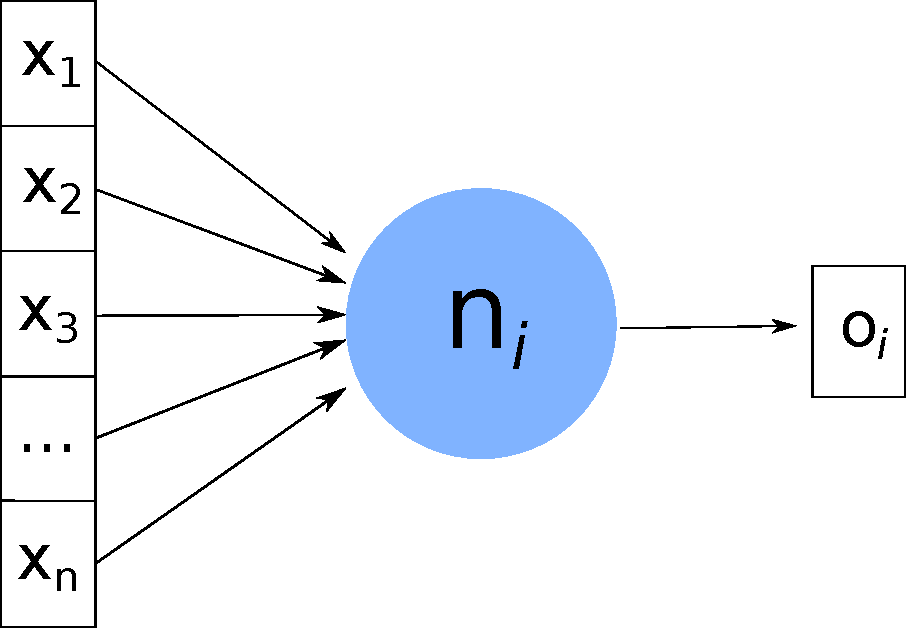
\includegraphics[width=0.8\textwidth]{images/neuron.pdf}
\end{figure}

\end{frame}


\begin{frame}{Background: Affine Transform Neurons}



\end{frame}

\begin{frame}{Background: Convolution Neurons}
\centering
\animategraphics[loop,controls,width=0.6\linewidth]{1}{images/arbitrary_padding_no_strides_0}{0}{3}
\end{frame}

\begin{frame}{Background: Layers}

\begin{figure}
    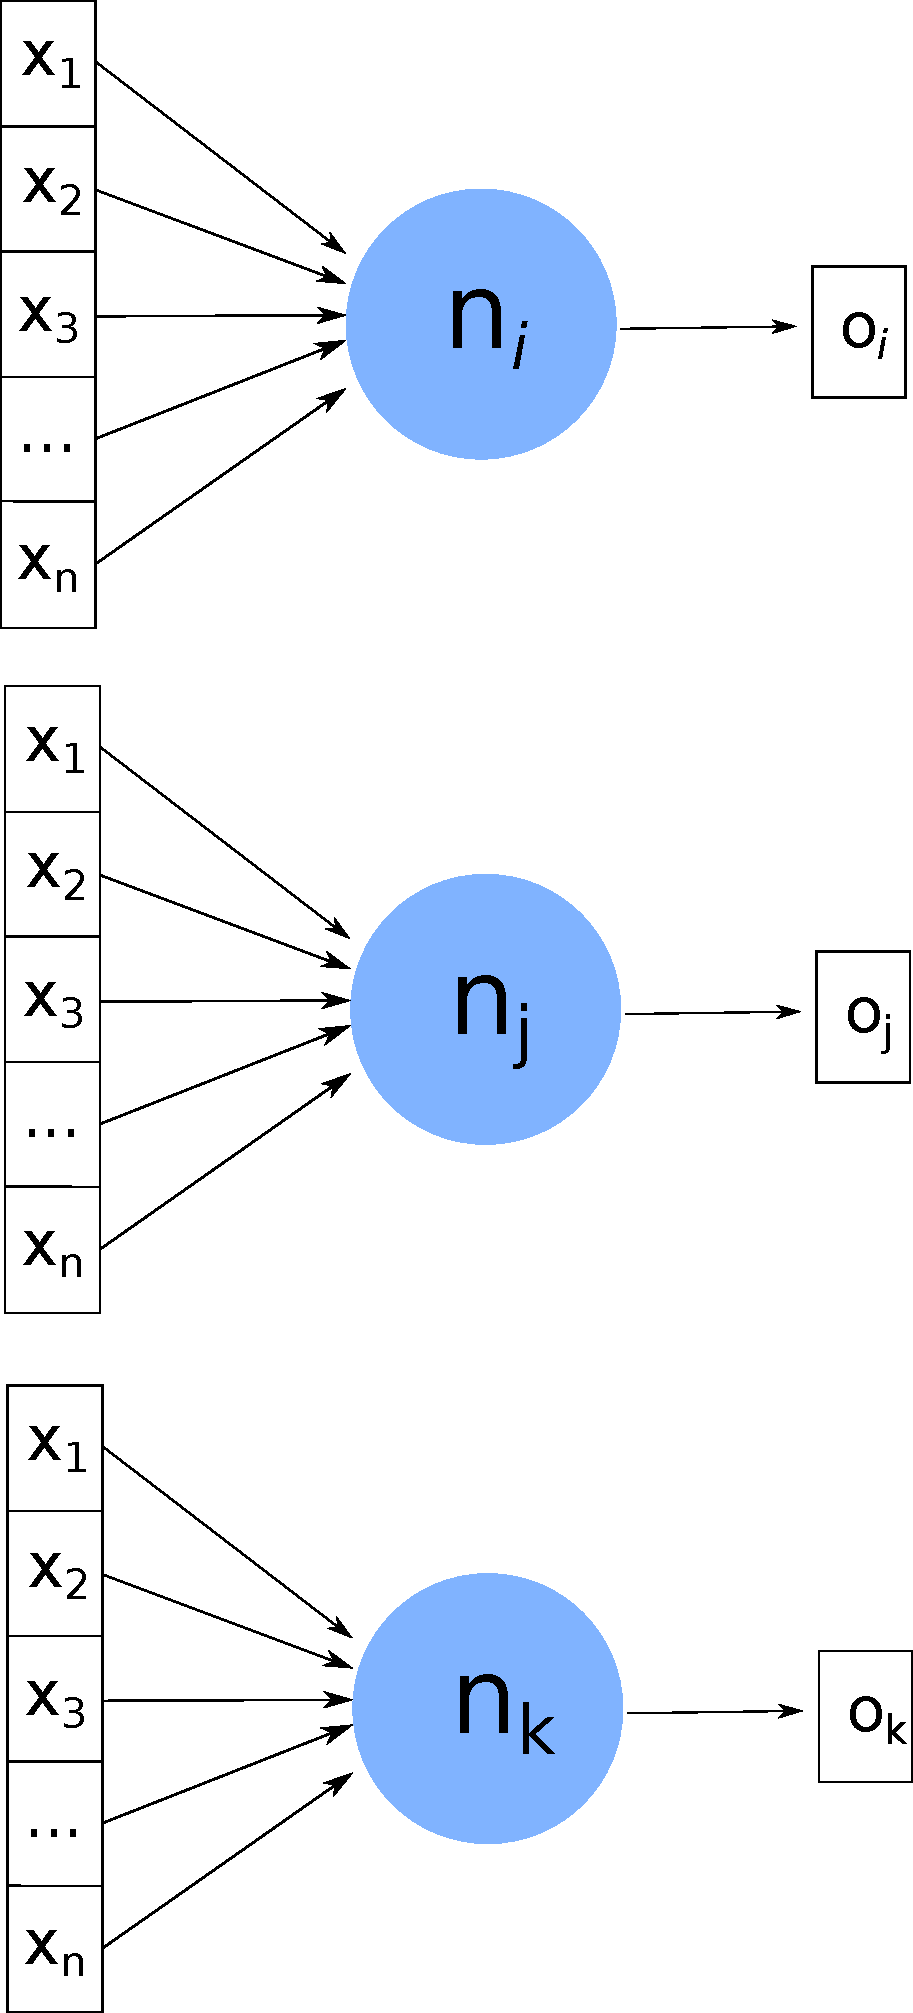
\includegraphics[width=3cm]{images/layer.pdf}
\end{figure}

\end{frame}


\begin{frame}{Background: Neural Networks}

\begin{figure}
    \centering
    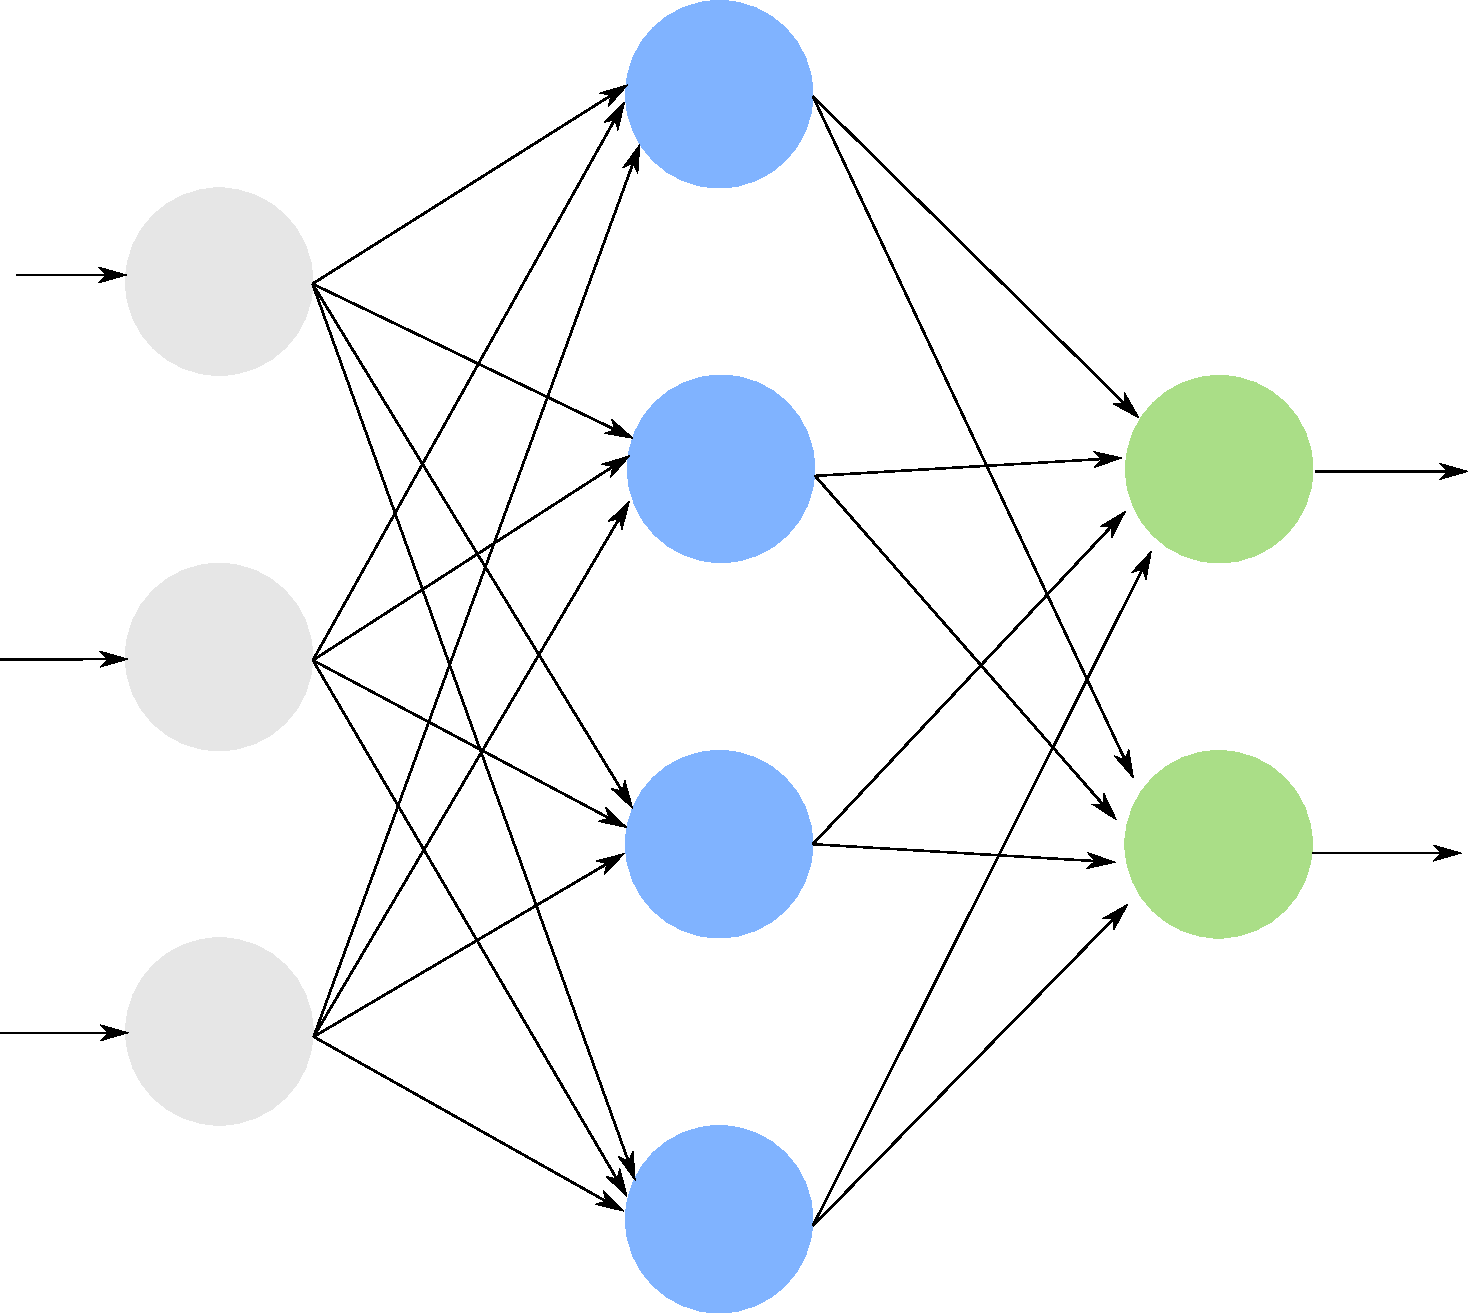
\includegraphics[width=0.6\linewidth]{images/neural_network.pdf}
\end{figure}
\end{frame}


\section{Inference Stack}

\begin{frame}{The Deep Learning Inference Stack}
\begin{figure}
    \centering
    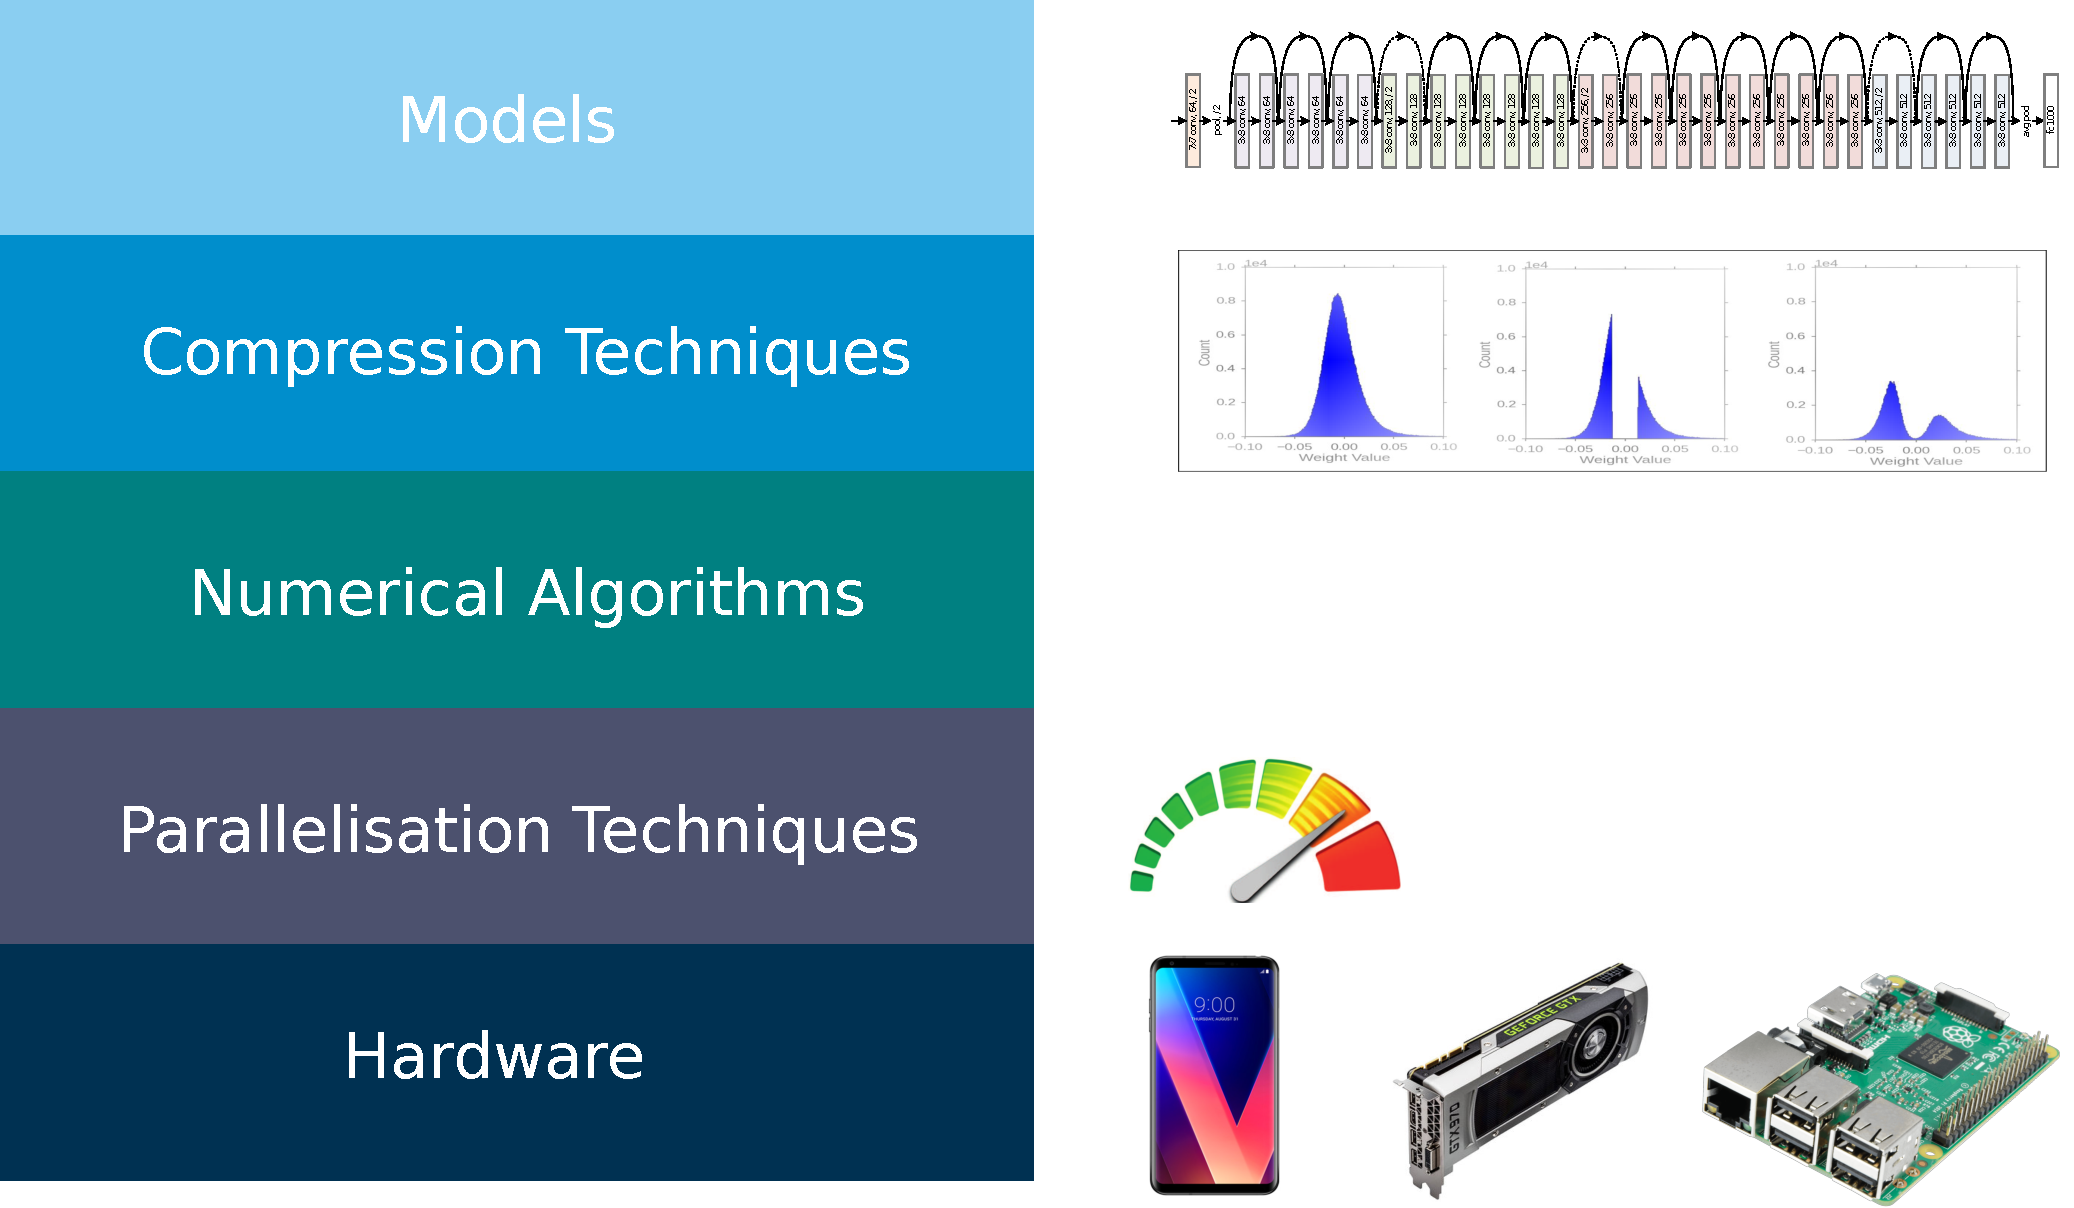
\includegraphics[width=\linewidth]{images/inference-stack.pdf}
    \caption{The Deep Learning Inference Stack}
    \label{fig:inference-stack}
\end{figure}
\end{frame}

\begin{frame}{Layer 1: Neural Networks}

\begin{columns}
\column{0.3\textwidth}

\begin{figure}
    \centering
    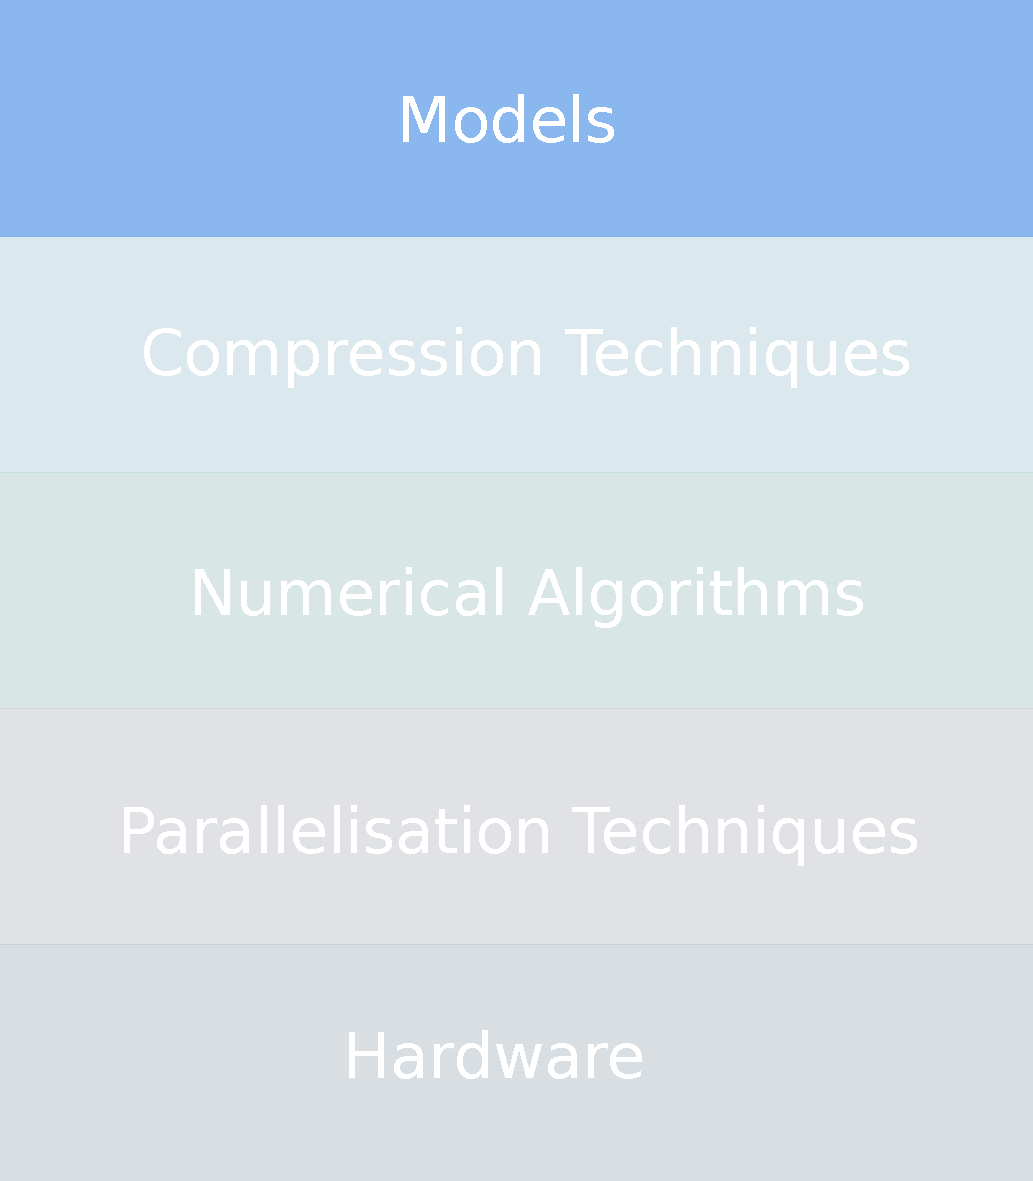
\includegraphics[width=3.5cm]{images/models.pdf}
    \label{fig:inference-stack-models}
\end{figure}

\column{0.7\textwidth}

\textbf{Neural Network Models}

\begin{itemize}
    \item Number of layers
    \item Number of neurons in each layer
    \item Operation each neuron performs
\end{itemize}

\begin{figure}
    \centering
    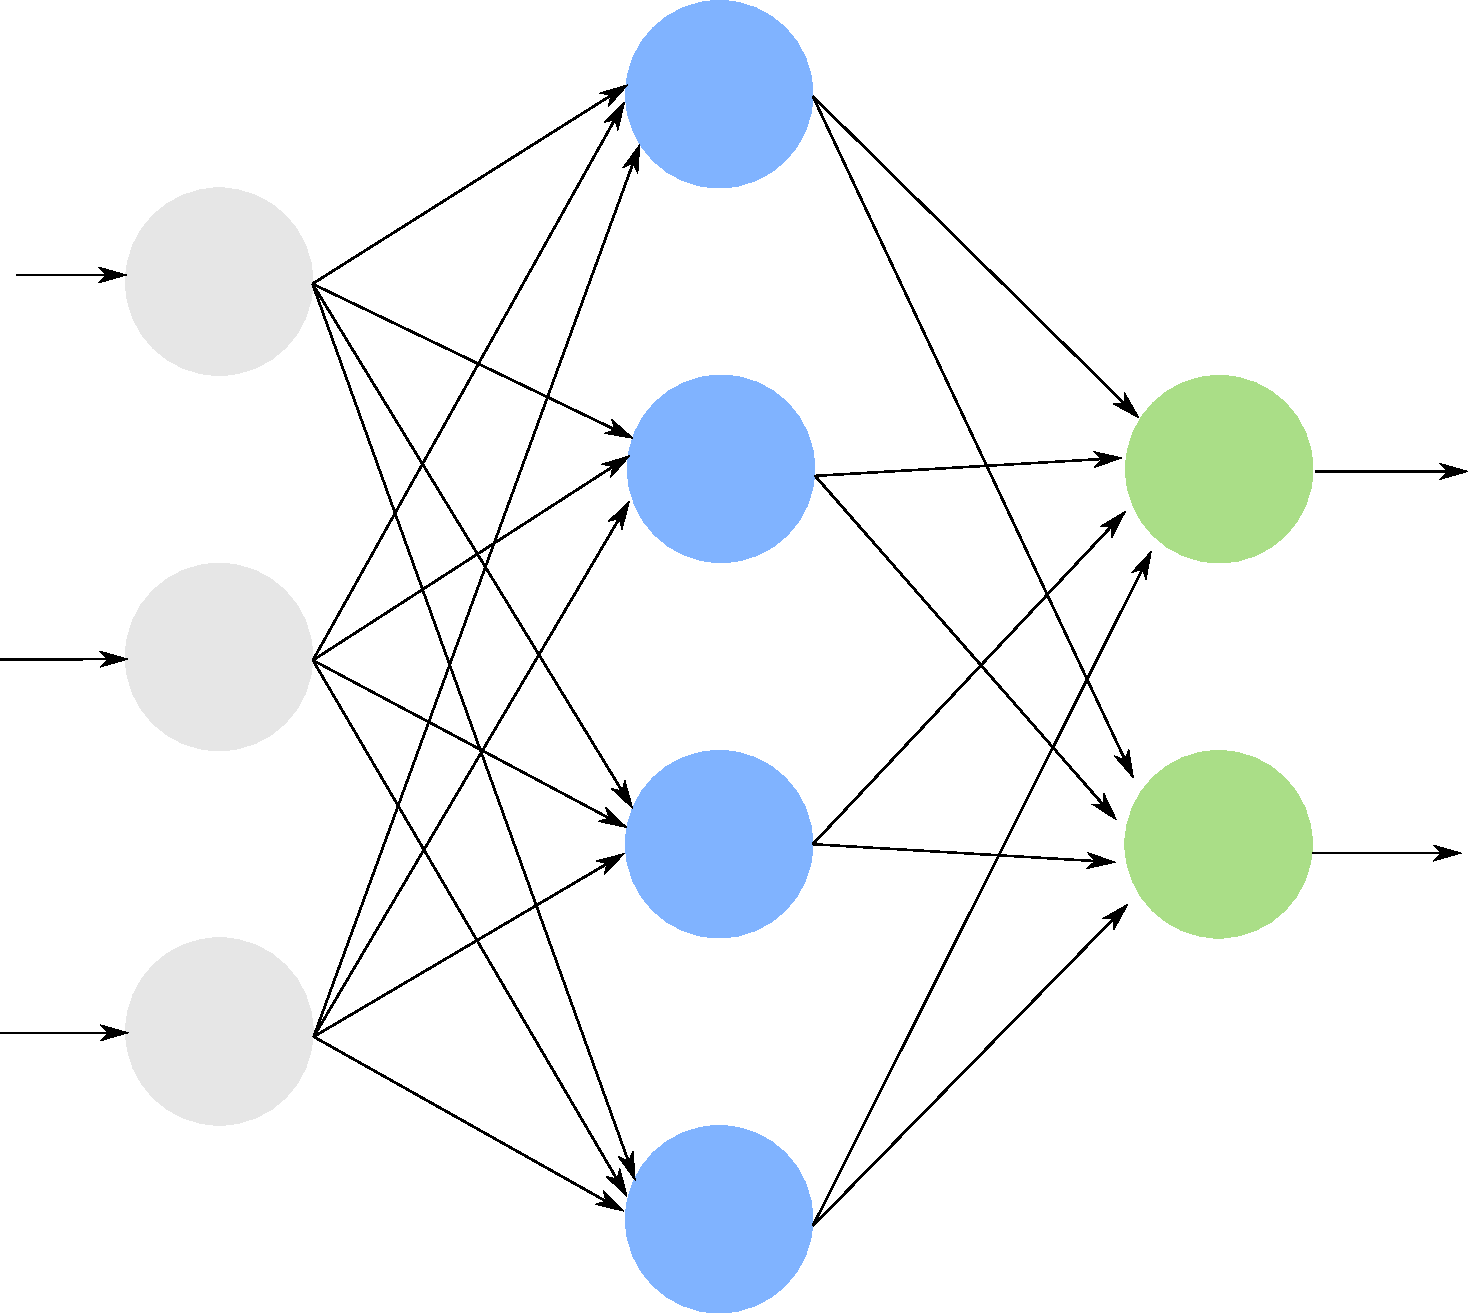
\includegraphics[width=5.5cm]{images/neural_network.pdf}
\end{figure}

\end{columns}


\end{frame}

\begin{frame}{Layer 2: Compression Techniques}

\begin{columns}
\column{0.3\textwidth}
\begin{figure}
    \centering
    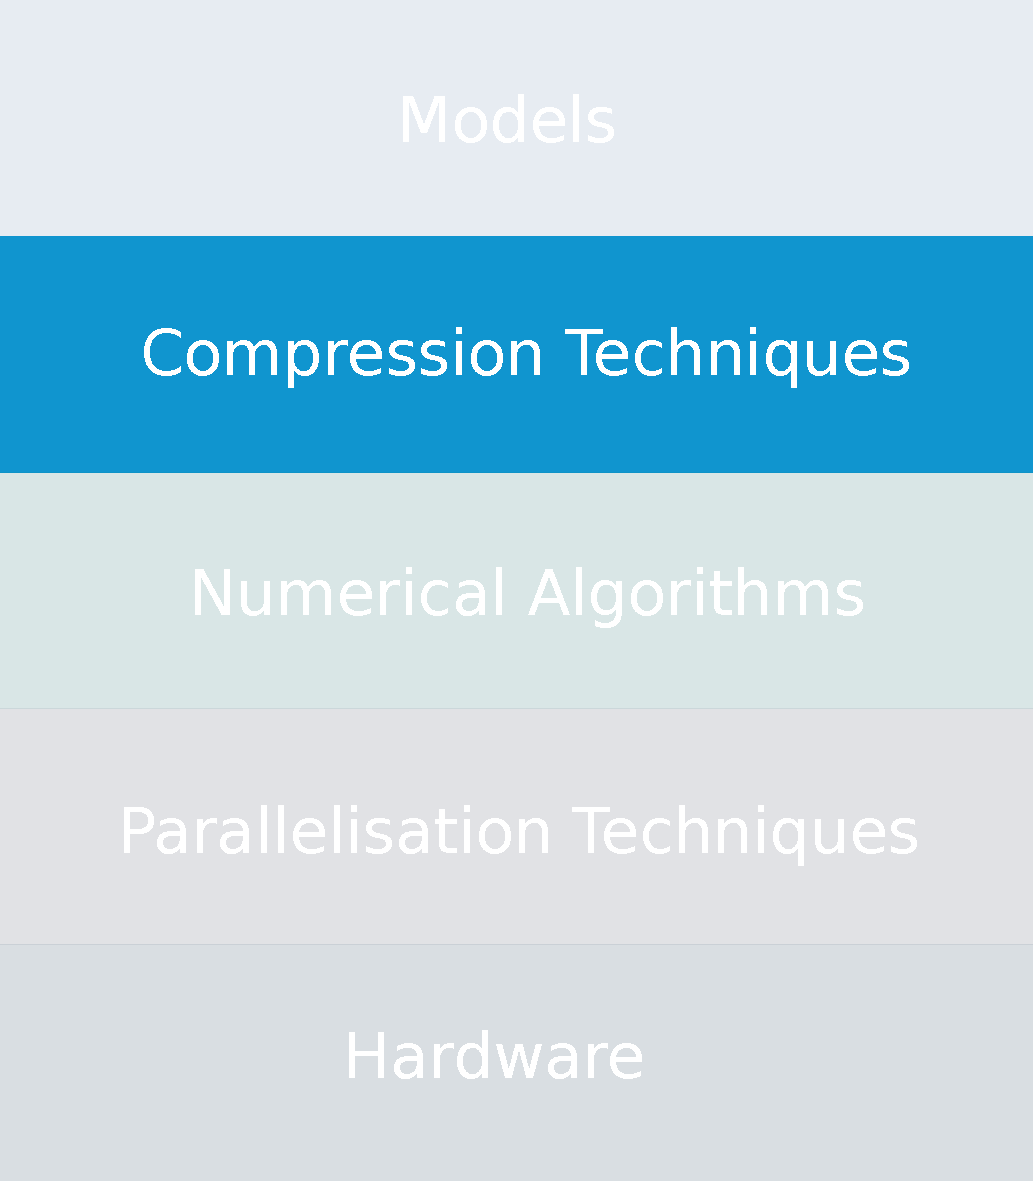
\includegraphics[width=3.5cm]{images/compressions.pdf}
    \label{fig:inference-stack-compress-1}
\end{figure}

\column{0.7\textwidth}

\textbf{Weight Pruning}

\begin{itemize}
    \item Pruning at the individual \textit{weight} level
    \item Leaves weight matrices very sparse
\end{itemize}

\begin{figure}
    \centering
    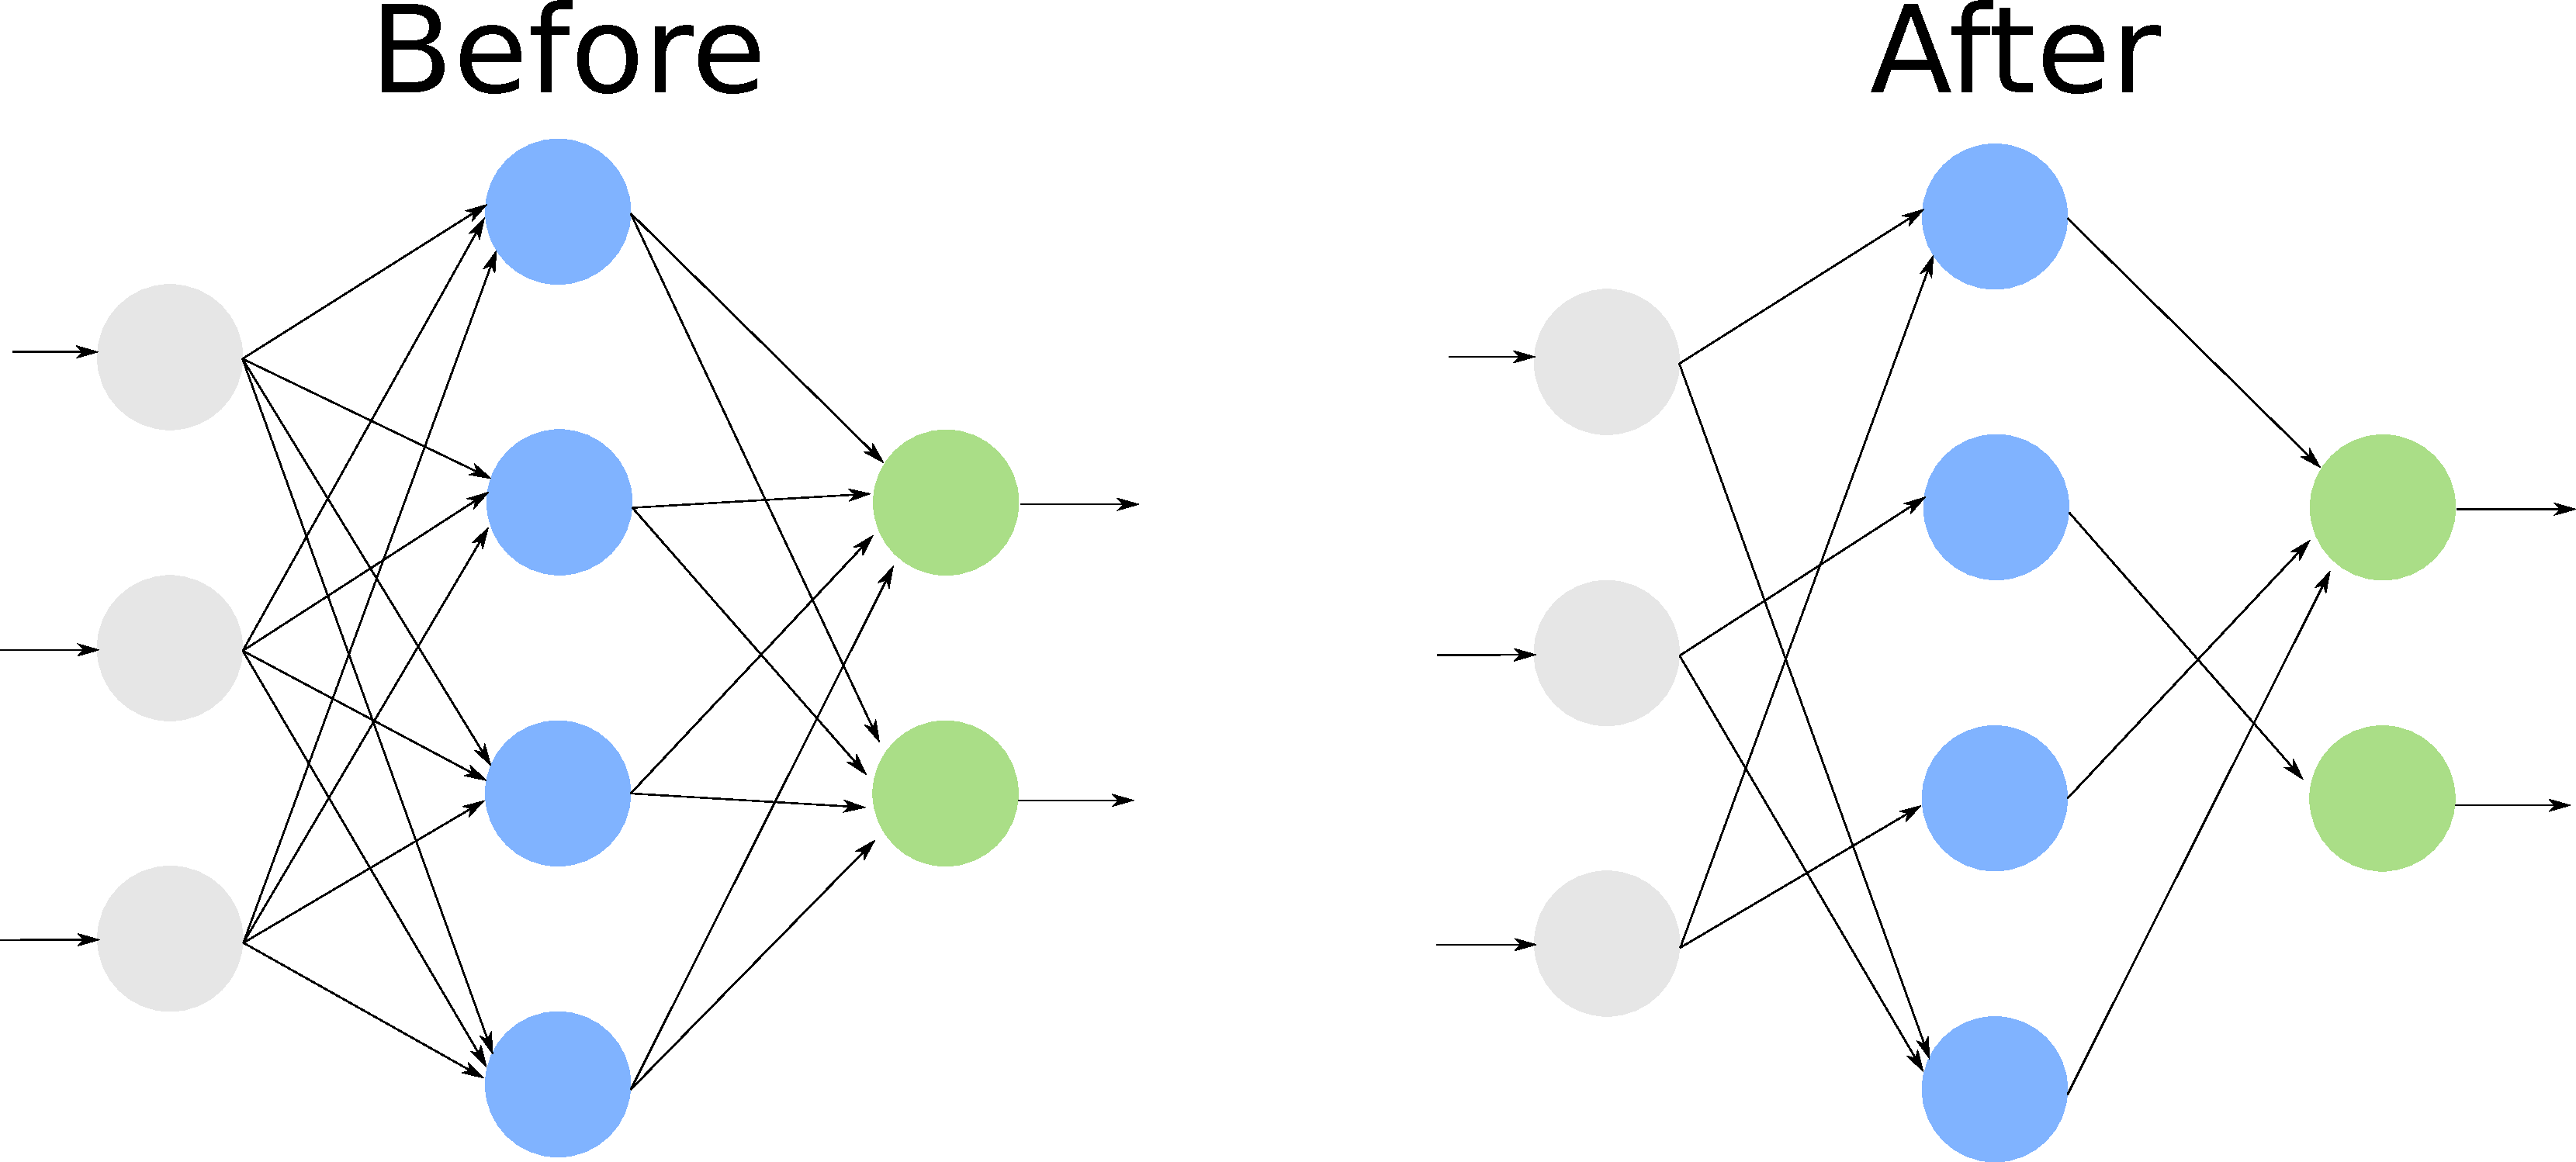
\includegraphics[width=6cm]{images/weight_pruning.pdf}
\end{figure}


\end{columns}

\end{frame}

\begin{frame}{Layer 2: Compression Techniques}

\begin{columns}

\column{0.3\textwidth}

\begin{figure}
    \centering
    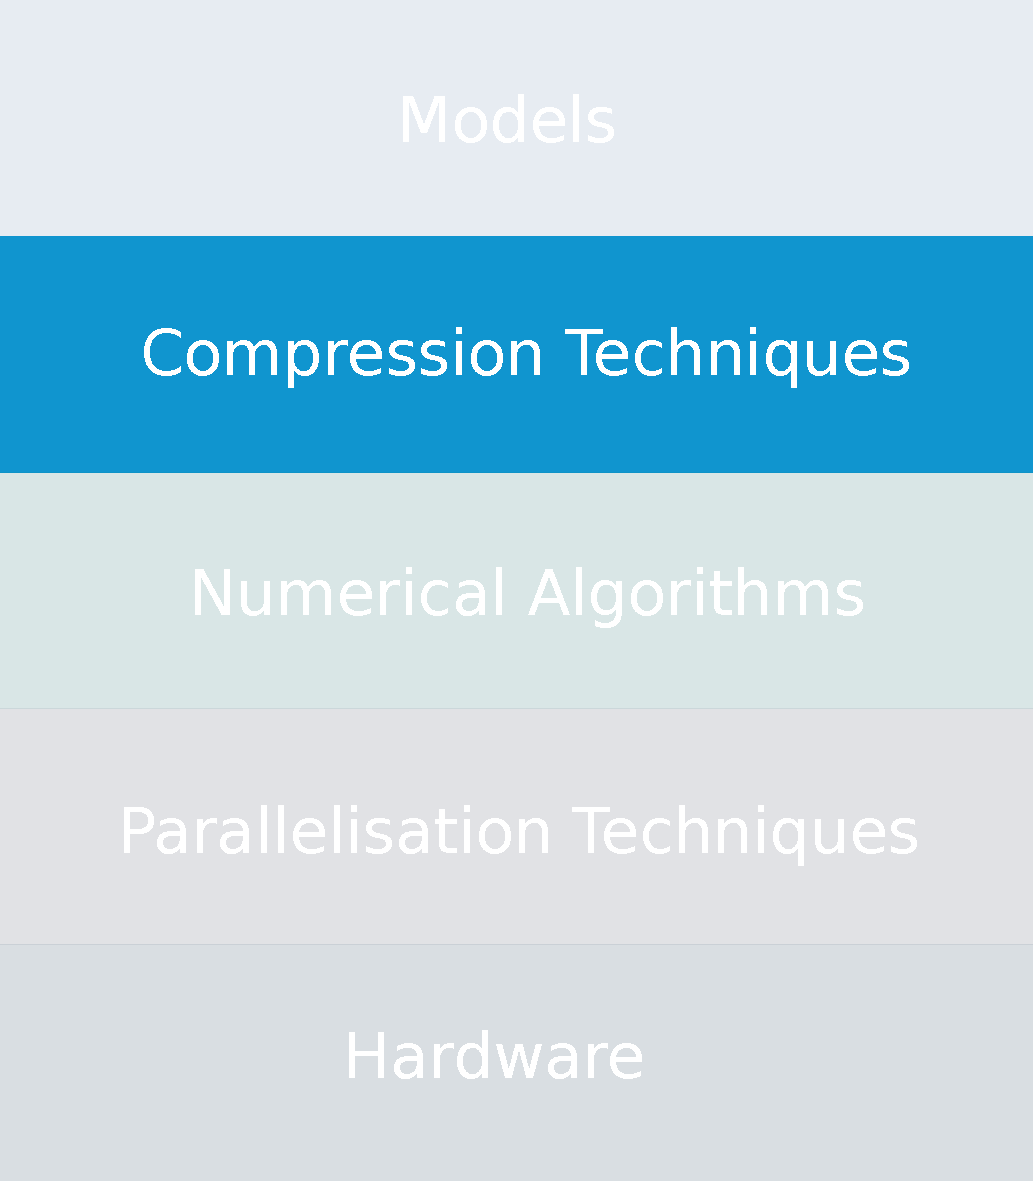
\includegraphics[width=3.5cm]{images/compressions.pdf}
    \label{fig:inference-stack-compress-2}
\end{figure}

\column{0.7\textwidth}

\textbf{Channel Pruning}
\begin{itemize}
    \item Pruning at the \textit{neuron} level
    \item Leaves matrices small and dense
\end{itemize}

\begin{figure}
    \centering
    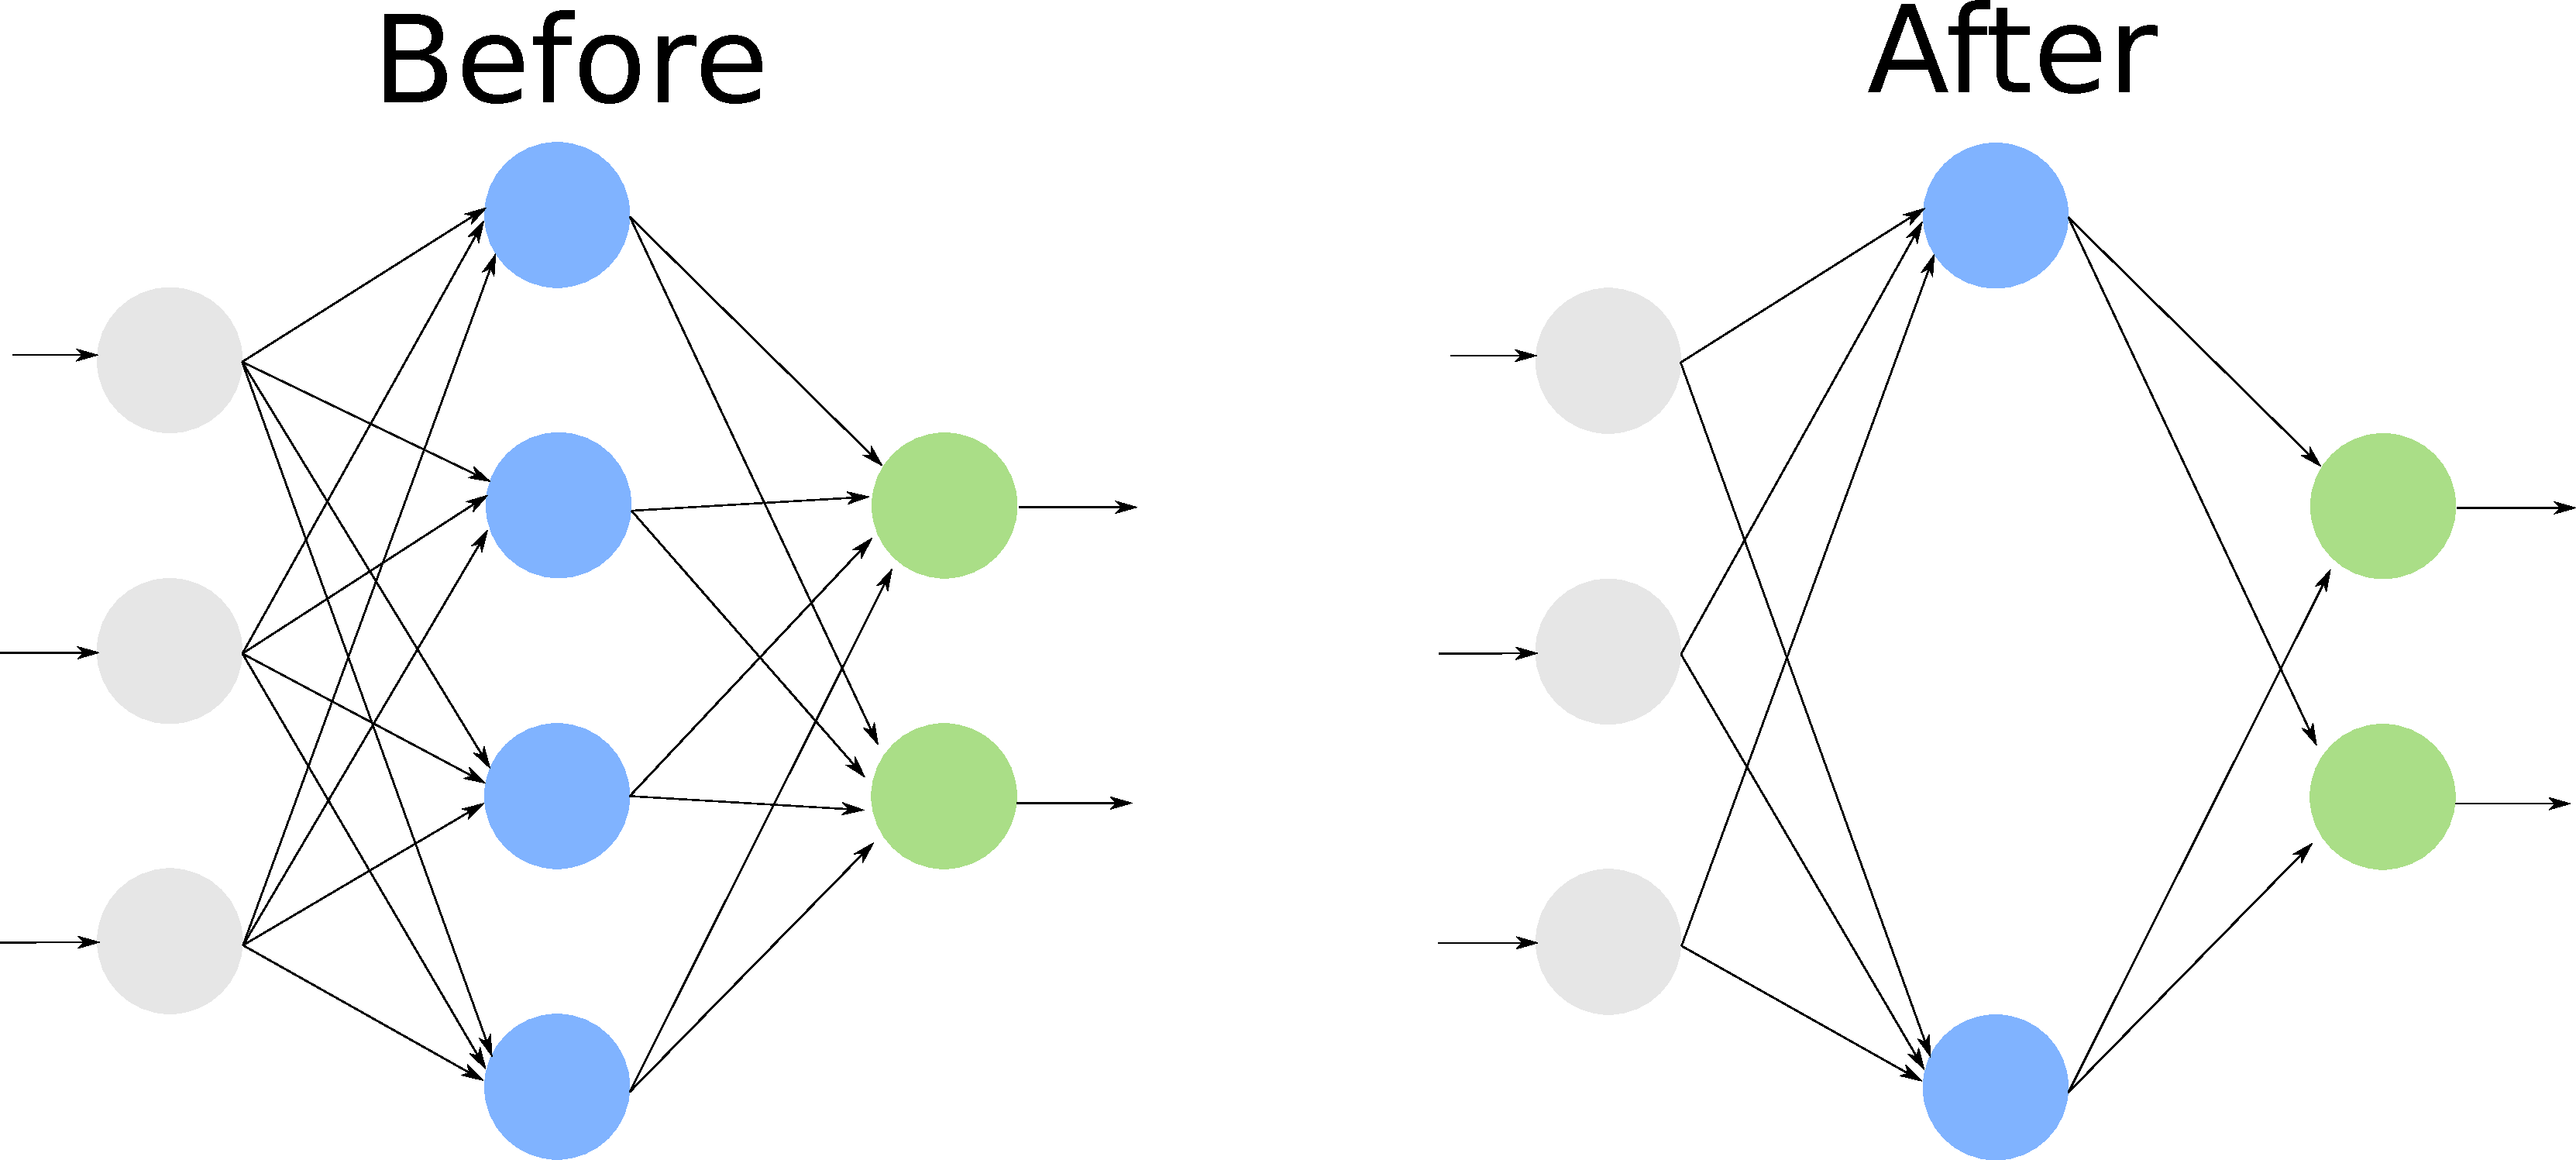
\includegraphics[width=6cm]{images/channel_pruning.pdf}
    \label{fig:channel_pruning}
\end{figure}

\end{columns}

\end{frame}

\begin{frame}{Layer 2: Compression Techniques}
\begin{columns}

\column{0.3\textwidth}
\begin{figure}
    \centering
    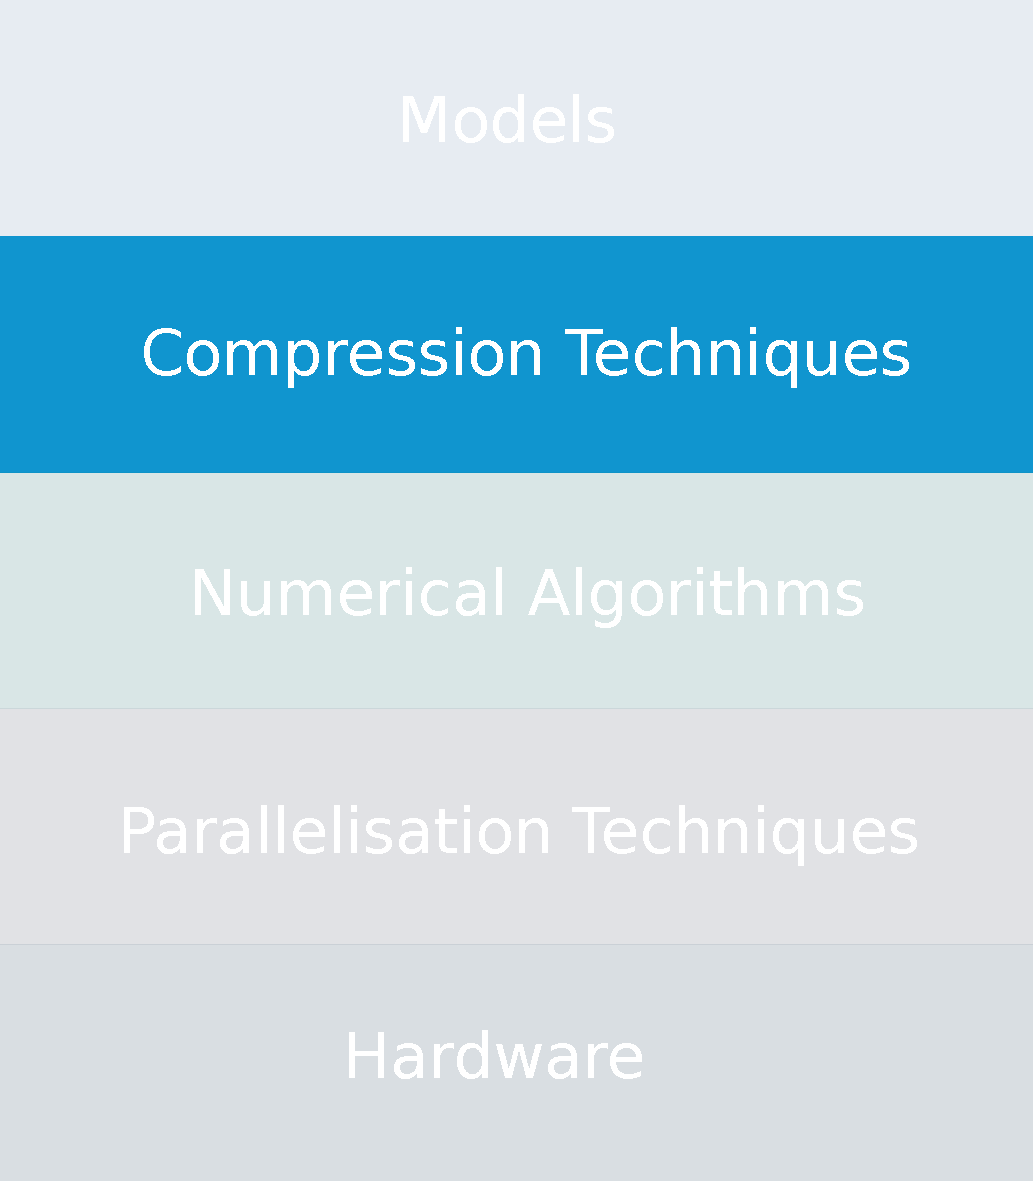
\includegraphics[width=3.5cm]{images/compressions.pdf}
    \label{fig:inference-stack-compress-3}
\end{figure}

\column{0.7\textwidth}

\textbf{Quantization}
\begin{itemize}
    \item Two options:
    \begin{enumerate}
        \item Reduce precision of weights
        \item Group to small set of centroids
    \end{enumerate}
\end{itemize}

\begin{figure}
    \centering
    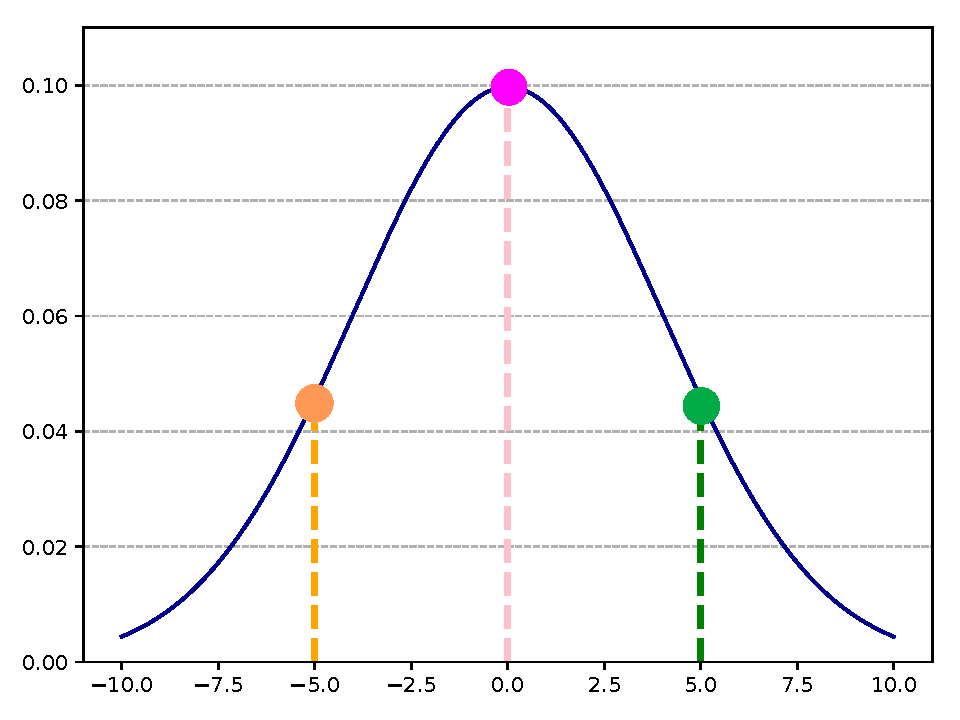
\includegraphics[width=5cm]{images/quantization.pdf}
\end{figure}

\end{columns}
\end{frame}



\begin{frame}{Layer 3: Numerical Algorithms}

\begin{columns}

\column{0.3\textwidth}
\begin{figure}
    \centering
    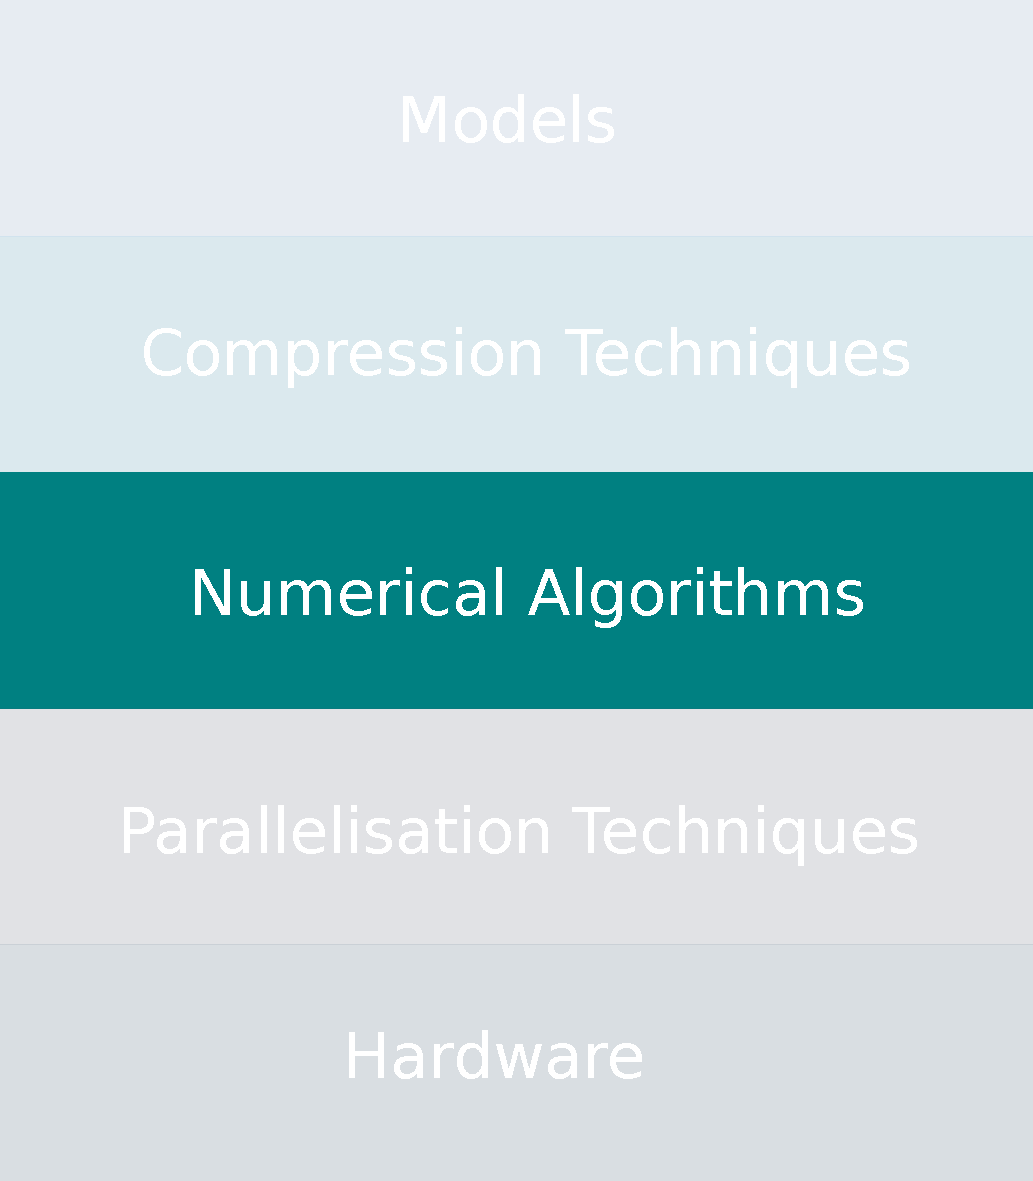
\includegraphics[width=3.5cm]{images/numericals.pdf}
    \label{fig:inference-stack-nums-1}
\end{figure}

\column{0.7\textwidth}

\begin{itemize}
    \item Direct convolution
    \item \texttt{im2col}
    \item FFT and Winograd
\end{itemize}

\end{columns}
\end{frame}


\begin{frame}{Layer 3: Numerical Algorithms}

\begin{columns}

\column{0.3\textwidth}

\begin{figure}
    \centering
    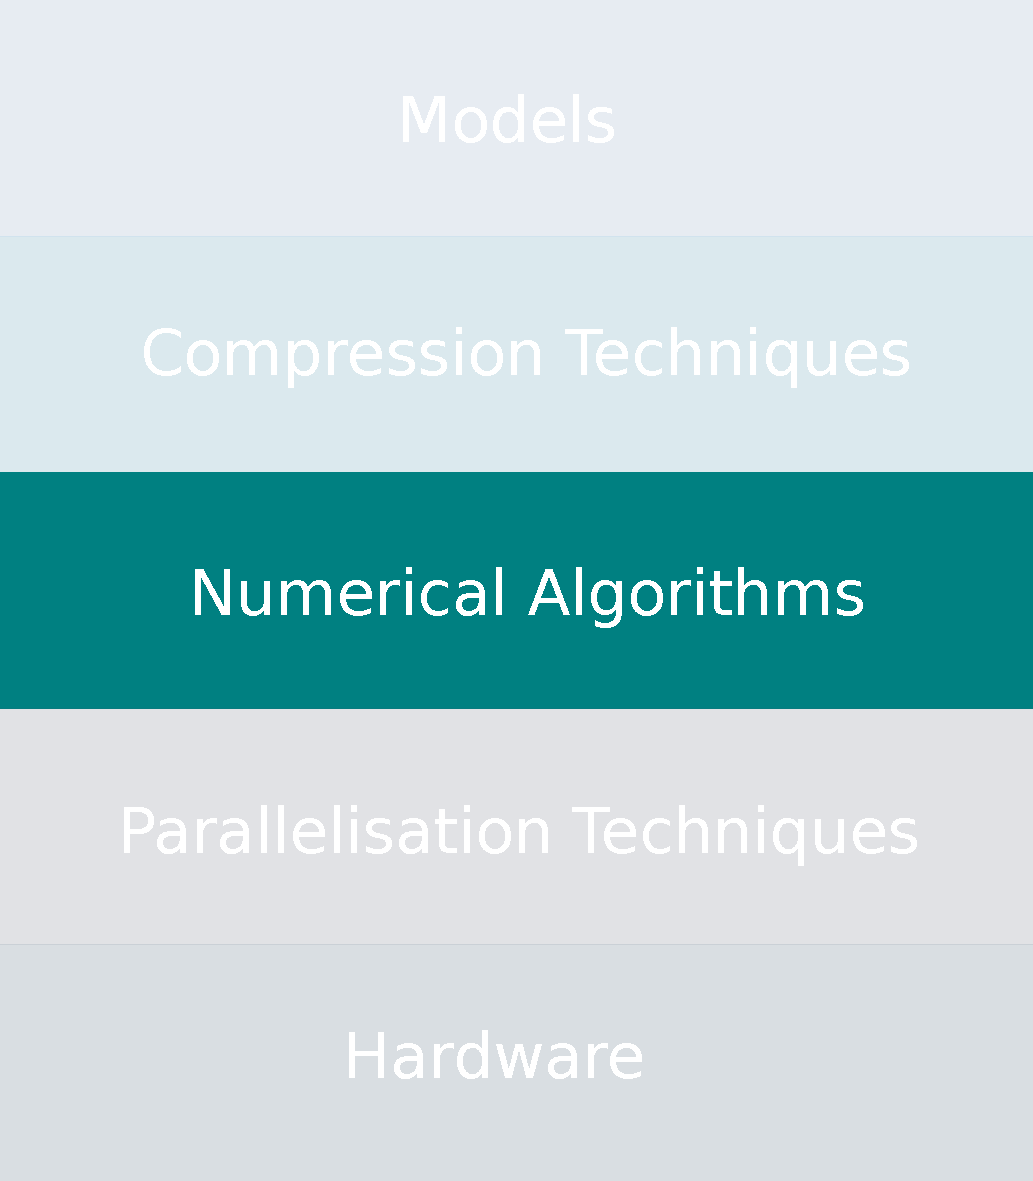
\includegraphics[width=3.5cm]{images/numericals.pdf}
    \label{fig:inference-stack-nums-2}
\end{figure}

\column{0.7\textwidth}
\begin{itemize}
    \item CSR
\end{itemize}

\end{columns}
\end{frame}

\begin{frame}{Layer 4: Parallelisation Techniques}

\begin{columns}


\column{0.3\textwidth}
\begin{figure}
    \centering
    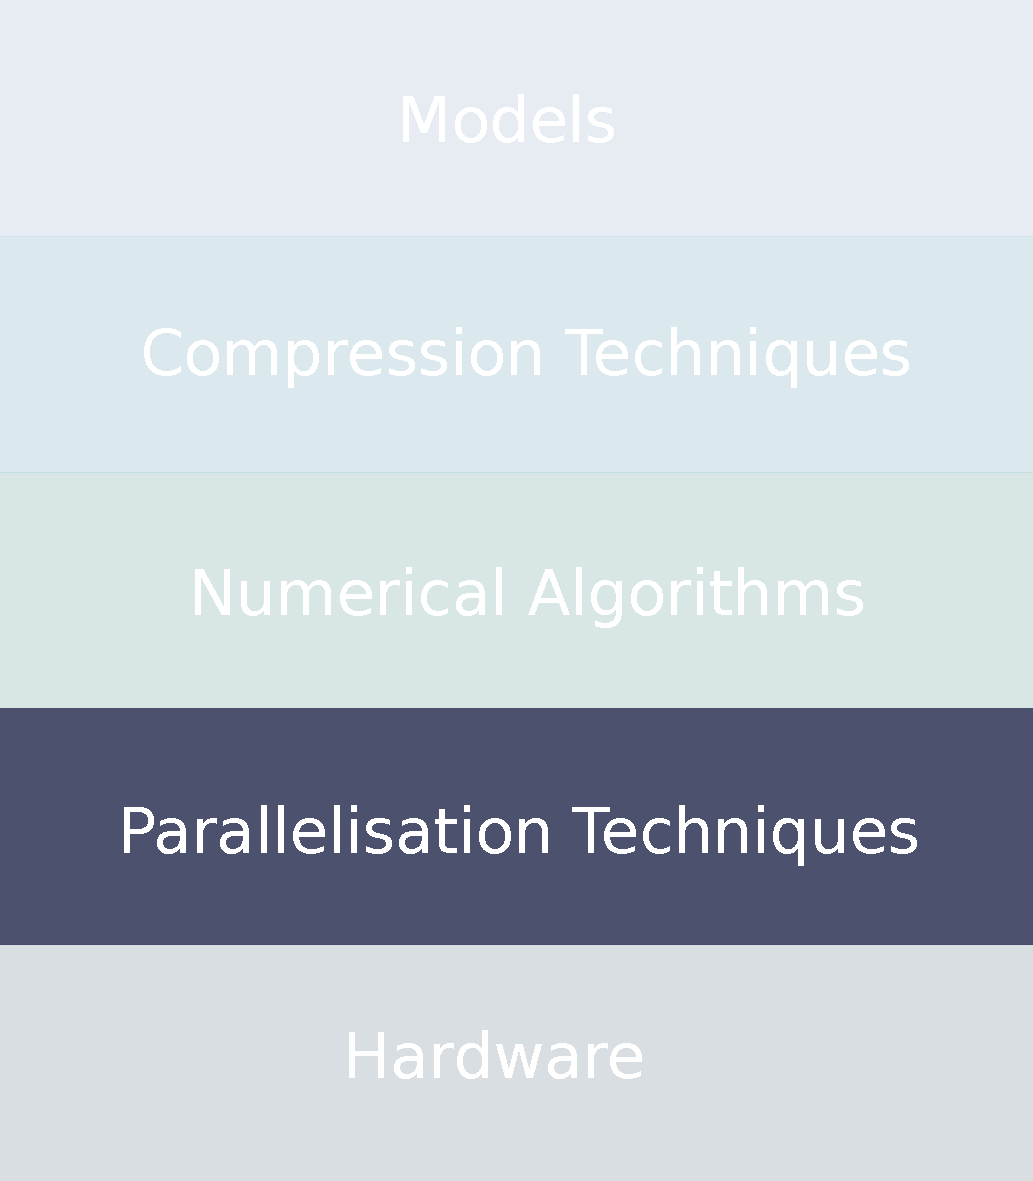
\includegraphics[width=3.5cm]{images/parallelisations.pdf}
    \label{fig:inference-stack-parallels}
\end{figure}

\column{0.7\textwidth}

\textbf{OpenMP}
\begin{itemize}
    \item CPU parallelisation of direct convolution 
    \item Something detailed about how OpenMP handles parallelisation
\end{itemize}

\end{columns}

\end{frame}


\begin{frame}{Layer 4: Parallelisation Techniques}

\begin{columns}


\column{0.3\textwidth}
\begin{figure}
    \centering
    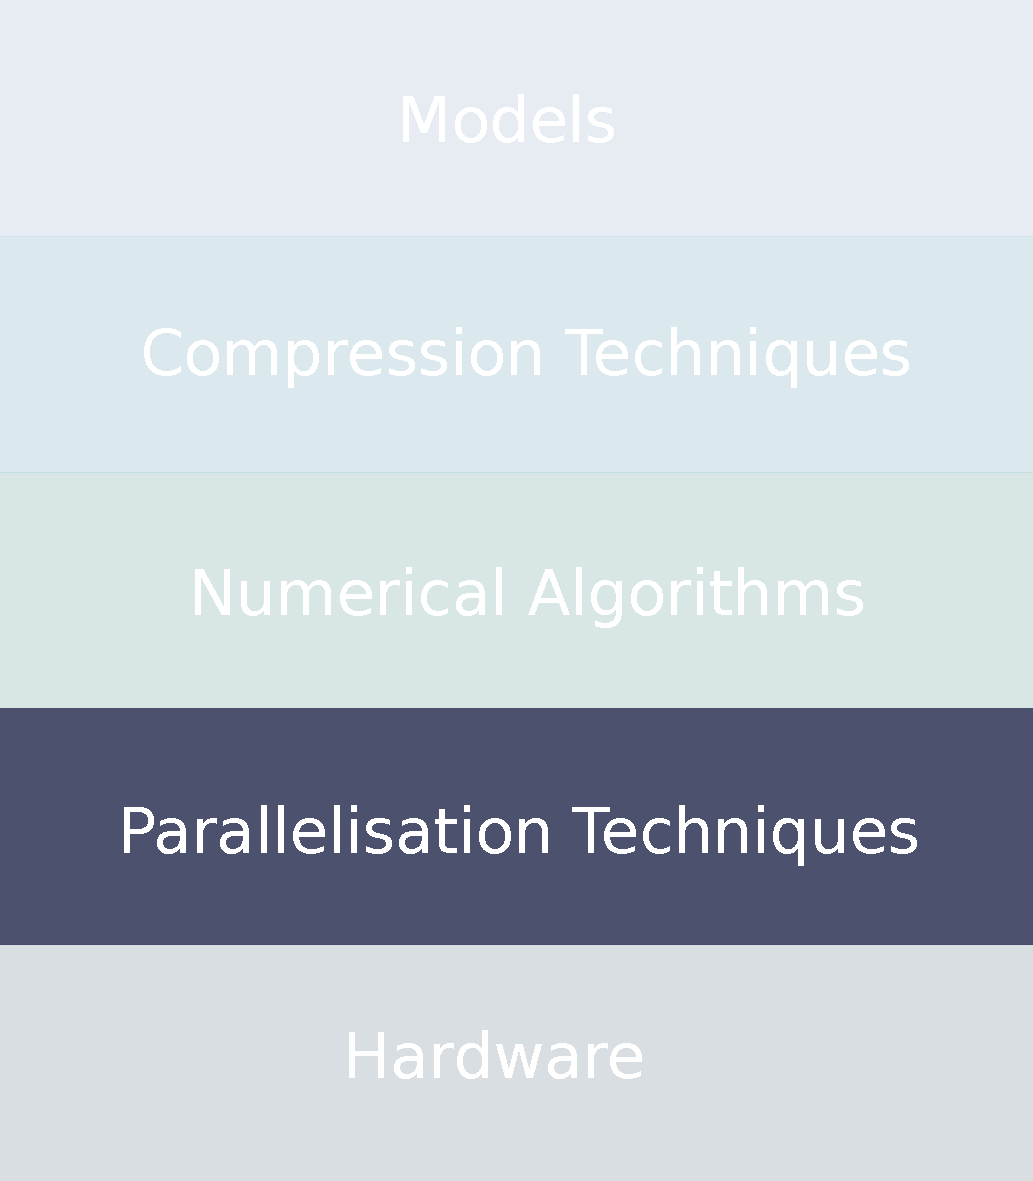
\includegraphics[width=3.5cm]{images/parallelisations.pdf}
    \label{fig:inference-stack-parallels-2}
\end{figure}

\column{0.7\textwidth}

\textbf{OpenCL}
\begin{itemize}
    \item Tile size
    \item Register blocking 
    \item CLBlast Autotuning 
\end{itemize}

\end{columns}

\end{frame}



\begin{frame}{Layer 5: Hardware}

\begin{columns}


\column{0.3\textwidth}
\begin{figure}
    \centering
    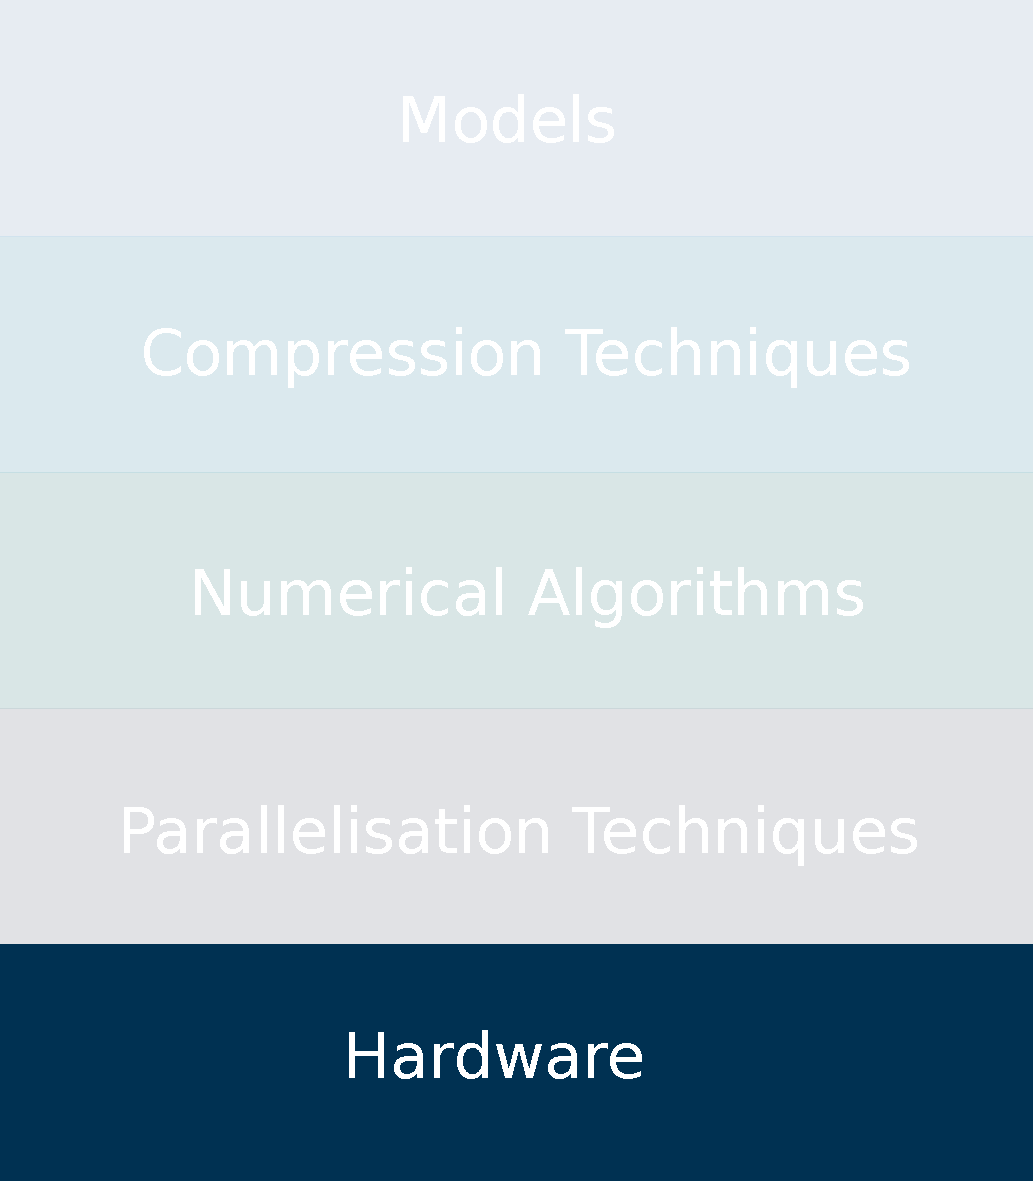
\includegraphics[width=3.5cm]{images/hardwares.pdf}
\end{figure}

\column{0.7\textwidth}

\begin{itemize}
    \item CPU
    \item GPU
    \item Typical embedded device setup
\end{itemize}
\end{columns}


\end{frame}





\end{document}
